% -*- mode: noweb; noweb-default-code-mode: R-mode; -*-
\documentclass[11pt, a4paper]{article}

%\VignetteIndexEntry{robustlmm: Robust Estimating Equations and Examples}
%\VignetteDepends{ggplot2, reshape2, xtable, robustlmm, digest}

\usepackage[a4paper, text={16cm,25cm}]{geometry}
\usepackage[utf8]{inputenc}
\usepackage{natbib}
\usepackage{amsmath,amssymb,amsthm}
\usepackage{graphicx}
\usepackage{multirow}

%% replace all tildes by hats
\renewcommand{\tilde}{\widehat}
\let\wtilde\widetilde
\renewcommand{\widetilde}{\widehat}

%% Some shortcuts
\newcommand{\abs}[1]    {\left| #1 \right|}
\newcommand*{\Rp}{\textsf{R}$\;$}
\newcommand{\T}[1]      {\texttt{#1}}
\newcommand{\fn}[1]{\kern-1pt\left(#1\right)\kern+0.5pt}
\newcommand{\fns}[1]{\kern-0.5pt(#1)}
\newcommand{\bld}[1]{\boldsymbol{#1}}
\renewcommand{\vec}[1]{\bld{#1}}
\newcommand{\vp}[1][e]{\Vec{\psi}_{#1}}
\newcommand{\tv}[2][]{{\widetilde{\vec{#2}}_{#1}}}
\newcommand{\hv}[2][]{{\widehat{\Vec{#2}}_{#1}}}
\newcommand{\s}[1][\rho]{#1^{(\sigma)}}
\newcommand{\si}[2][w]{#1^{(\sigma)}_{#2}\kern-1pt}
\newcommand{\vbs}{\vec b^{*}}
\newcommand{\vbstr}{\vec b^{*\intercal}}
\newcommand{\tvbs}{\widetilde{\vec{b}}^{\raisebox{-0.75ex}{\scriptsize *}}}
\newcommand{\hvbs}{\widehat{\vec{b}}^{\raisebox{-0.75ex}{\scriptsize *}}}
\newcommand{\hvbstr}{\widehat{\Vec{b}}^{\raisebox{-0.3ex}{\scriptsize\ensuremath{*\intercal}}}}
\newcommand{\bs}{b^{*}}
\newcommand{\bsQ}{b^{*2}}
\newcommand{\hbs}{\widehat{b}^{*}}
\newcommand{\es}{\varepsilon^{*}}
\newcommand{\ves}{\vec\varepsilon^{*}}
\newcommand{\tves}{\widetilde{\vec{\varepsilon}}^{\raisebox{-0.75ex}{\scriptsize *}}}
\newcommand{\hves}{\widehat{\vec{\varepsilon}}^{\raisebox{-0.75ex}{\scriptsize *}}}
\newcommand{\hes}{\widehat{\varepsilon}^{*}}
\newcommand{\U}[2][-0.15ex]{\bld{U}_{\hspace{#1}#2\hspace{0.25ex}}}
\newcommand{\V}[2][-0.15ex]{\bld{V}_{\hspace{#1}#2\hspace{0.25ex}}}
\newcommand{\Ue}{\U{e}}
\newcommand{\Ub}{\U{b}}
\newcommand{\Ubth}{\U{b}\fn{\vec\theta}}
\newcommand{\Vbth}{\V{b}\fn{\vec\theta}}
\newcommand{\W}[1][b]{\text{\textbf{W}}_{\hspace{-0.5ex}#1\hspace{0.25ex}}}
\newcommand{\w}[2][b]{w_{#1}^{(#2)}}
\newcommand{\kbtau}{\kappa_b^{(\tau)}}
\newcommand{\tr}{^{\intercal}}
\newcommand{\trinv}{^{-\raisebox{0.3ex}{\scriptsize$\intercal$}}}
\newcommand{\invsq}{^{-1/2}}
\newcommand{\diag}{\mbox{\textbf{Diag}}}
\newcommand{\ERWSymbol}{\mathbb{E}}
\newcommand{\makeright}[2]{\ifx#1\left\right#2\else#1#2\fi}
\newcommand{\Xsub}[2]{{#1}_{\mathrm{\scriptscriptstyle #2}}}
\newcommand{\ERW}[2][\left] {\ERWSymbol    #1[ #2 \makeright{#1}{]}}
\newcommand{\ERWi}[3][\left] {\Xsub{\ERWSymbol}{#2}    #1[ #3
    \makeright{#1}{]}}
\newcommand{\Tbk}{\bld{T}_{\hspace{-0.5ex}b,k\hspace{0.25ex}}}
\newcommand{\Q}[1]{\bld{Q}_{\hspace{-0.15ex}{#1}}}
\newcommand{\Qlkhth}{\Q{l,k}\fns{\hv\theta}}
\newcommand{\Qlhth}{\Q{l}\fns{\hv\theta}}
\DeclareMathOperator{\N}{\mathcal{N}}
\DeclareMathOperator{\trace}{tr}
\DeclareMathOperator{\eff}{eff}
\DeclareMathOperator{\sign}{sign}

%% Sweave stuff
\usepackage{color}
\usepackage{Sweave}
\definecolor{Sinput}{rgb}{0,0,0.56}
\definecolor{Soutput}{rgb}{0.56,0,0}
\DefineVerbatimEnvironment{Sinput}{Verbatim}{%
formatcom={\color{Sinput}}, fontsize=\footnotesize}
\DefineVerbatimEnvironment{Soutput}{Verbatim}{%
formatcom={\color{Soutput}}, fontsize=\footnotesize}
\fvset{listparameters={\setlength{\topsep}{0pt}}}
\renewenvironment{Schunk}{\vspace{\topsep}}{\vspace{\topsep}}

%% Set width of plots
\setkeys{Gin}{width=\textwidth}

%% remark environment
\newtheoremstyle{note}% name
  {3pt}%      Space above
  {3pt}%      Space below
  {\small}%         Body font
  {\parindent}%         Indent amount (empty = no indent, \parindent = para indent)
  {\itshape}% Thm head font
  {.}%        Punctuation after thm head
  {.5em}%     Space after thm head: " " = normal interword space;
        %       \newline = linebreak
  {}%         Thm head spec (can be left empty, meaning `normal')

\theoremstyle{note}
\newtheorem*{remark}{Remark}
\newtheorem*{remarks}{Remarks}

%% hyperreferences
\usepackage{hyperref}
\hypersetup{
    colorlinks,
    citecolor=black,
    filecolor=black,
    linkcolor=black,
    urlcolor=black
}

\begin{document}

\author{Manuel Koller\\[1em]
  \small{Seminar f\"ur Statistik, ETH Z\"urich}\\
  \small{and}\\
  \small{Institute of Social and Preventive Medicine, University of Bern}}
\title{\T{robustlmm}: Robust Estimating Equations and Examples}
\maketitle

This vignette attempts to give some background on the robust estimation
method implemented in ``rlmer''. Moreover, two example analyses are
included that aim to facilitate the first time user to start working with
this package. The text presented here is basically a summary of
\citet{koller2013}. In said reference, a detailed derivation of the methods
underlying ``rlmer'' can be found.

The model and some notation is introduced in Section~\ref{sec:model}. The
robust estimating equations are given in Section~\ref{sec:eeq}. Then two
examples are analyzed in Sections \ref{sec:penicillin} and
\ref{sec:sleepstudy}. Both datasets are also analyzed in
\citet{bates2011lme4}. For the convenience of the reader, the description
of the datasets found there has been included here. Finally, in
Section~\ref{sec:tc} we provide tables of tuning constants and the
definition of the \emph{smoothed Huber $\psi$-function}.

\section{The Model}
\label{sec:model}
Following \citet{bates2011lme4}, we work with the formulation
of mixed effects models in terms of spherical random effects,
\begin{equation}
  \label{eq:mixedModelSpherical}
  \begin{split}
    \vec y = \bld X\vec\beta + \bld Z\Ubth\vbs + \Ue\ves\;, \\
    \vbs \sim \bld{\N}\fn{\vec 0, \sigma^2\bld I_q}\;, \quad
    \ves \sim \bld{\N}\fn{\vec 0, \sigma^2\bld I_n}\;, \quad
    \vbs \perp \ves\;,
  \end{split}
\end{equation}
where $q$ is the number of random effects (the length of $\vbs$) and $n$ is
the number of observations (length of $\vec y$). The vector $\vec\theta$
parametrizes the lower triangular part $\Ubth$ of the Cholesky
decomposition of the covariance matrix of the random effects $\Vbth$, i.e.,
$\Vbth = \Ubth\Ubth\tr$. We assume the random effects to be ordered in a
way such that correlated random effects are grouped togheter. The
covariance matrix $\Vbth$ is therefore block diagonal. We use the index $i$
for observations, $j$ for random effects and $k$ for blocks of random
effects. For notatinal simplicity, we assume that there is only one type of
blocks. Generalizing the estimating equations given below is
straightforward and left to the reader.

\section{Robust Estimating Equations}
\label{sec:eeq}
\subsection{Fixed and Random Effects}
Let $k\fn{j}$ be a function that maps random effect $j$ to the
corresponding block $k$, then the squared Mahalanobis distances of the
estimated random effects are
\begin{equation*}
  \vec d = \left(d\fn{b_{k\fn{j}}/\sigma}\right)_{j=1,\dots,q}\;,
  \quad \mbox{where} \quad
  d\fn{b_k} = \vbstr_k\vbs_k\;.
\end{equation*}
Then we may define the robustness weight for the $j$th random effect as
$w_b\fns{d_j}$. We use standard (location and linear regression) robustness
weights:
\begin{equation*}
    w_b\fn{d} = \left\{
      \begin{array}{cl}
        {\psi_b\fn{\sqrt{d}}}/\sqrt{d} & \mbox{ if } d \neq 0\;, \\
        \psi_b'\fn{0} & \mbox{ if } d = 0\;.
      \end{array}
    \right.
\end{equation*}
It is convenient to represent the robustness weights as (diagonal)
weighting matrix,
\begin{equation*}
  \W\fn{\vec d} =
  \diag\fn{w_b\fn{d_{k\fn{j}}}}_{j=1,\dots,q}\;.
\end{equation*}
The robust estimating equations are then
\begin{equation}
  \label{eq:robustEEq}
  \begin{split}
    \bld X\tr\Ue\trinv \bld\psi_e\fn{{\tves}/{\sigma}}
    = {} & 0\;, \\
    \Ub\tr\bld Z\tr\Ue\trinv \bld\psi_e\fn{{\tves}/{\sigma}} -
    \bld\Lambda_b \W\fn{\tv d}{\tvbs}/{\sigma}
    = {} & 0\;,
  \end{split}
\end{equation}
where $\bld\Lambda_b = \diag\fn{\lambda_{e}/\lambda_{b,j}}_{j=1,\dots,q}$
is a diagonal matrix with elements depending on the block size
$s_{k\fn{j}}$, $\lambda_e = \ERWi{0}{\psi'_e\fn{\es}}$ and
$\lambda_{b,j} = \wtilde\lambda\fn{s_{k\fn{j}}}$,
\begin{equation*}
  \wtilde\lambda\fn{s} = \ERWi{0}{\frac{\partial}{\partial \bs_1}
    \left(
      w_b\fn{\vbstr\vbs}\vbs_1
  \right)}\; \quad \vbs \sim \bld{\N}\fn{\vec 0, \bld I_s}\;.
\end{equation*}

\subsection{Scale}
We apply the Design Adaptive Scale approach following \citet{ks2011}. We get
\begin{equation}
  \label{eq:sigmaDAS}
  \sum_{i=1}^n\tau_{e,i}^2\si{e}\fn{\frac{\hes_i}{\tau_{e,i}\widehat\sigma}}
  \left[
    \left(\frac{\hes_i}{\tau_{e,i}\widehat\sigma}\right)^2 - \s[\kappa]_e
  \right] = 0\;,
\end{equation}
where the superscript $\s[\cdot]$ is used to distinguish the weighting
functions used for the scale and covariance parameters from the ones for the
fixed effects. Just as in the linear regression case, we define
$\tau_{e,i}$ as the value that zeroes the expectation of the $i$-th summand
in \eqref{eq:sigmaDAS}. The expectation is
\begin{equation}
  \label{eq:tau_ei}
  \ERW{\si{e}\fn{\frac{\hes_i}{\tau_{e,i}\widehat\sigma}}
    \left(\frac{\hes_i}{\tau_{e,i}\widehat\sigma}\right)^2 -
    \s[\kappa]_e \si{e}\fn{\frac{\hes_i}{\tau_{e,i}\widehat\sigma}}} = 0\;,
\end{equation}
where the distribution of the residuals is approximated using a linear
expansion of $\tv\beta$ and $\tvbs$ around their true values
\citep[Appendix~C]{koller2013}, and $\s[\kappa]_e$ is
\begin{equation*}
  \s[\kappa]_e =
  {\ERWi{0}{\si{e}\fn{\varepsilon}\varepsilon^2}}\Big/
  {\ERWi{0}{\si{e}\fn{\varepsilon}}}\;.
\end{equation*}

The weighting functions used for the scale estimates are the squared
robustness weights used for the estimation of the fixed and random effects,
$\si{e}\fns{x} = (\si[\psi]{e}\fns{x}/x)^2$, $\si{e}\fns{0} =
\si[\psi]{e}'\fns{0}$, for convex $\rho$-functions. For redescending
$\rho$-functions, it is not necessary to use the squared robustness
weights, using the same weights as for the fixed and random effects still
gives robust estimates (assuming $\psi\fns{x}x$ is bounded). When using the
squared weights, it is crucial to use a different set of tuning parameters
for estimating the scale and covariance parameters. Tables of tuning
parameters can be found in Section~\ref{sec:tc}.

\subsection{Covariance Parameters}
For the covariance parameters, we have to treat the diagonal and the
non-diagonal $\Ub$ case separately.

\subsubsection{Diagonal Case}
In the case of diagonal $\Ubth$, the estimation of $\tv\theta$ is
essentially a scale estimation problem on $\tvbs$. It can be robustified
just like the estimating equation for $\hat\sigma$ \eqref{eq:sigmaDAS}. The
robust estimating equations are
\begin{equation}
  \label{eq:thetaDAS}
  \sum_{j=1}^q\tau_{b,j}^2\si{b}\fn{\frac{\hbs_j}{\tau_{b,i}\widehat\sigma}}
  \left[
    \left(\frac{\hbs_j}{\tau_{b,j}\widehat\sigma}\right)^2 - \s[\kappa]_b
  \right] = 0\;,
\end{equation}
with $\tau_{b,i}$ such that
\begin{equation*}
  %\label{eq:tau_bi}
  \ERW{\si{b}\fn{\frac{\hbs_i}{\tau_{b,i}\widehat\sigma}}
    \left[\left(\frac{\hbs_i}{\tau_{b,i}\widehat\sigma}\right)^2 -
    \s[\kappa]_b\right]} = 0\;,
\end{equation*}
and normalizing constant
\begin{equation*}
  \s[\kappa]_b = {\ERWi{0}{\si{b}\fn{\bs}\bsQ}}\Big/
  {\ERWi{0}{\si{b}\fn{\bs}}}\;.
\end{equation*}

\subsubsection{Non-diagonal Case}
For non-diagonal $\Ubth$ we have to take care of the block structure. The
normalizing constant $\tau_{b,i}^2$ has to be replaced by a matrix $\Tbk$
which is defined for each block $k$. Analogue to the estimator for the
covariance matrix and location problem, we have to use two different weight
functions, one for the size of the matrix $\w{\tau}$ and another one for
the shape $\w{\eta}$. For details, we refer to \citet{stahel1987estimation}
and \citet[Chapter~5]{HamFRRS86}. As is done in the cited references, we
introduce a third weight function $\w{\delta}$ to simplify notation. For
block types with dimension $s > 1$, let
\begin{equation*}
  \w{\delta}\fn{d} = \left(d\w{\eta}\fn{d} -
    \left(d-s\kbtau\right)\w{\tau}\fn{d-s\kbtau}\right)\Big/s\;,
\end{equation*}
where $\kbtau$ is defined such that
\begin{equation*}
  \ERW{\left(u - s\kbtau\right)\w{\tau}\fn{u - s\kbtau}} = 0 \quad
  \mbox{for }u\sim\chi^2_s.
\end{equation*}

\begin{remark}
  The optimal $B$-robust estimator derived in \citet{stahel1987estimation}
  is given by $\w{\tau}\fn{d} = \min\fn{1/b_\tau, 1/d}$ and $\w{\eta}\fn{d}
  = \min{\fn{1/b_\eta, 1/d}}$. Other weight functions may be chosen, as
  long as $\psi\fn{d} = dw\fn{d}$ is a $\psi$-function. For $\w{\tau}$ and
  $\w{\eta}$ given above, this would be the Huber $\psi$-function. For low
  dimensions $s$ one may choose $\w{\tau} = \w{\eta}$. In higher
  dimensions, the efficiency loss for the estimated size is negligible.
  Hence one may choose a smaller tuning parameter for $\w{\eta}$. For
  $s=2$, and Huber or smoothed Huber $\psi$-functions (see
  Section~\ref{sec:tc}), one may use the squared tuning parameter of $\s_e$
  for $\w{\tau}$ to get approximately the same efficiency for $\hv\theta$
  as for $\widehat\sigma$.  Tables of tuning parameters for higher
  dimensions for the Huber and the lqq $\psi$-functions can be found in
  Section~\ref{sec:tc}.
\end{remark}

The robust estimating equation in the non-diagonal case can then be defined
as follows. For $l = 1,\dots,r$,
\begin{equation}
  \label{eq:thetaDASNonDiag}
  \begin{split}
    \sum_{k=1}^K\bigg[
    \w{\eta}\fn{d\fn{{\Tbk\invsq\hvbs_k}/{\widehat\sigma}}}
    \hvbstr_k\Qlkhth\hvbs_k/{\widehat\sigma^2} \qquad\qquad\qquad\qquad \\
    - \w{\delta}\fn{d\fn{{\Tbk\invsq\hvbs_k}/{\widehat\sigma}}}
    \trace\fn{\Tbk\Qlkhth} \bigg] =
    0\;,
  \end{split}
\end{equation}
where $\Qlkhth$ is the $s\times s$ submatrix of $\Qlhth$ which acts on
block $k$ and $\Tbk\invsq$ is the inverse of any square root of the
$s\times s$ matrix $\Tbk$. As in the diagonal case, we define the matrix
$\Tbk$ such that each summand has expectation zero. For $l = 1, \dots, r$,
\begin{equation*}
  \begin{split}
    \ERWSymbol\bigg[\w{\eta}\fn{d\fn{{\Tbk\invsq\hvbs_k}/{\sigma}}}
    \hvbstr_k\Qlkhth\hvbs_k/{\sigma^2} \qquad\qquad\qquad\qquad\quad \\
    - \w{\delta}\fn{d\fn{{\Tbk\invsq\hvbs_k}/{\sigma}}}
    \trace\fn{\Tbk\Qlkhth} \bigg] = 0\;.
  \end{split}
\end{equation*}
\begin{remarks}
  The symmetric matrix $\Tbk$ is fully defined for unstructured covariance
  matrices only, where $r = s(s+1)/2$. For other covariance matrix
  structures we can replace $\Tbk$ by the variance of the linear
  approximation of $\vbs$.

  Since in the classical case, the linear approximations for $\hvbs$ and
  $\hves$ are exact, the estimating equation \eqref{eq:thetaDASNonDiag}
  reduces to the REML estimating equations. A similar argument is valid for
  the estimating equation for $\hat\sigma$ \eqref{eq:sigmaDAS}.
\end{remarks}

%% Initialize Sweave


%\SweaveOpts{eval=FALSE}


\section{Penicillin Example}
The dataset, shown in Figure~\ref{fig:penicillinRaw}, was originally
published by \citet{davies72penicillin}. They describe it as data coming
from an investigation to
\begin{quote}
  assess the variability between samples of penicillin by the
  \emph{B.~subtilis} method.  In this test method a bulk-inoculated
  nutrient agar medium is poured into a Petri dish of approximately 90
  mm.\ diameter, known as a plate.  When the medium has set, six small
  hollow cylinders or pots (about 4 mm.\ in diameter) are cemented onto
  the surface at equally spaced intervals.  A few drops of the
  penicillin solutions to be compared are placed in the respective
  cylinders, and the whole plate is placed in an incubator for a given
  time.  Penicillin diffuses from the pots into the agar, and this
  produces a clear circular zone of inhibition of growth of the
  organisms, which can be readily measured.  The diameter of the zone
  is related in a known way to the concentration of penicillin in the
  solution.
\end{quote}
The datasets contains the measurements of $6$ samples and $24$ plates.

\label{sec:penicillin}

\begin{figure}[htbp]
  \centering
  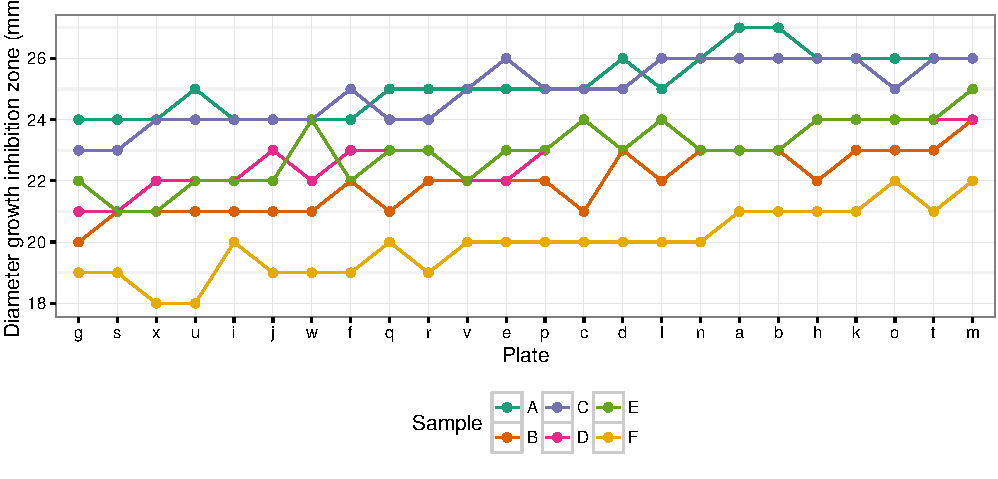
\includegraphics{figs/fig-ex-penicillin-raw}
  \caption{Diameters of growth inhibition zones of 6 samples applied to
    each of 24 agar plates to assess penicillin concentration in the
    \emph{B. subtilis} method. The lines join the observations of the same
    sample. The plates have been reordered by their means.}
  \label{fig:penicillinRaw}
\end{figure}

The raw data for the Penicillin example is shown in
Figure~\ref{fig:penicillinRaw}.  In \Rp, the data is provided as part of
the \Rp package ``lme4''. It is a data.frame with three columns:

\begin{Schunk}
\begin{Sinput}
> str(Penicillin)
\end{Sinput}
\begin{Soutput}
'data.frame':	144 obs. of  3 variables:
$ diameter: num 27 23 26 23 23 21 27 23 ...
$ plate : Factor w/ 24 levels "g","s","x","u",..: 18 18 18 18 18 18 19 19 ...
$ sample : Factor w/ 6 levels "A","B","C","D",..: 1 2 3 4 5 6 1 2 ...
\end{Soutput}
\end{Schunk}

The column ``diameter'' is the response and the two factors ``plate'' and
``sample'' indicate where the observation was measured. As
\citet{bates2011lme4}, we fit a linear mixed effects model with an
intercept and two random effects for the two factors.

We fit the classical linear mixed effects model using the function ``lmer''
of the \Rp package ``lme4''. The random effects are specified in
brackets. The pipe symbol ``|'' is used to split the factors and
covariables from the grouping variable. In this case, we only have a random
intercept ``1'' that varies by group ``plate'' and ``sample'',
respectively.

\begin{Schunk}
\begin{Sinput}
> st(classical <- lmer(diameter ~ 1 + (1|plate) + (1|sample),
+                      Penicillin))
\end{Sinput}
\end{Schunk}
\begin{Schunk}
\begin{Soutput}
   user  system elapsed 
  0.098   0.002   0.099 
\end{Soutput}
\end{Schunk}



The ``st'' function is just a shortcut to ``system.time'', a function that
measures the time required to evaluate the expression given as argument.

The robust mixed effects model is fit using the function ``rlmer''. The
call is quite similar to ``lmer'''s call. By default, it uses the smoothed Huber
$\psi$-function with tuning parameter $k=1.345$ and $s=10$. Since we are
mainly interested in the estimates of the variance components, we adjust
the the tuning parameter for the $\s[\psi]_.$ functions to $k = 2.28$ and
specify that squared weights are used. This makes sure that the variance
components are estimated with an efficiency of about $95\%$. One can do this
with one call to the function ``psi2propII''. Afterwards, we have a look
at the summary of the fitted object

\begin{Schunk}
\begin{Sinput}
> st(robust <- rlmer(diameter ~ 1 + (1|plate) + (1|sample), Penicillin,
+                    rho.sigma.e = psi2propII(smoothPsi, k = 2.28),
+                    rho.sigma.b = psi2propII(smoothPsi, k = 2.28)))
\end{Sinput}
\begin{Soutput}
   user  system elapsed 
 10.235   0.089  10.346 
\end{Soutput}
\begin{Sinput}
> summary(robust)
\end{Sinput}
\begin{Soutput}
Robust linear mixed model fit by DAStau 
Formula: diameter ~ 1 + (1 | plate) + (1 | sample) 
   Data: Penicillin 

Random effects:
 Groups   Name        Variance Std.Dev.
 plate    (Intercept) 0.7582   0.8707  
 sample   (Intercept) 3.8865   1.9714  
 Residual             0.2997   0.5475  
Number of obs: 144, groups: plate, 24; sample, 6

Fixed effects:
            Estimate Std. Error t value
(Intercept)  23.0419     0.8464   27.22

Robustness weights for the residuals: 
 124 weights are ~= 1. The remaining 20 ones are summarized as
   Min. 1st Qu.  Median    Mean 3rd Qu.    Max. 
  0.397   0.670   0.837   0.809   0.955   0.993 

Robustness weights for the random effects: 
 25 weights are ~= 1. The remaining 5 ones are
    1     2     3    24    30 
0.836 0.836 0.938 0.802 0.858 

Rho functions used for fitting:
  Residuals:
    eff: smoothed Huber (k = 1.345, s = 10) 
    sig: smoothed Huber, Proposal II (k = 2.28, s = 10) 
  Random Effects, variance component 1 (plate):
    eff: smoothed Huber (k = 1.345, s = 10) 
    vcp: smoothed Huber, Proposal II (k = 2.28, s = 10) 
  Random Effects, variance component 2 (sample):
    eff: smoothed Huber (k = 1.345, s = 10) 
    vcp: smoothed Huber, Proposal II (k = 2.28, s = 10) 
\end{Soutput}
\end{Schunk}

The first half of the summary shows information about the model that was
fitted and displays the parameter estimates including standard errors for
the fixed effects. After that, a summary of the robustness weights is
shown. In this case, we can see that some of the observations have been
downweighted, but practically none of the random effects. Finally there is
a table that gives details about which $\psi$-functions were used to fit
the model.
\begin{remark}
  Note that the column ``Std.Dev.'' contains the estimated standard
  deviances, i.e., just the square roots of the estimated variances. A
  common mistake is to interpret them as the standard errors of the
  variance component estimates. The same table is shown for the summary of
  an lme4 object and to ease the transition from ``lmer'' to ``rlmer'', we use the
  same convention here.
\end{remark}

Alternatively, one might be interested in a model that does not downweight
the random effects of ``sample'' -- for example because there might be
structural outliers and one is interested in the variability including
these. To enable this, ``rlmer'' accepts list input for the arguments
``rho.b'' and ``rho.sigma.b''. The list entries correspond to the
$\psi$-functions used for the variance components as shown in the summary
output. The call to fit a model that does uses the classical estimates for
the ``sample'' variance components is as follows.

\begin{Schunk}
\begin{Sinput}
> st(robust2 <- rlmer(diameter ~ 1 + (1|plate) + (1|sample), Penicillin,
+                     rho.sigma.e = psi2propII(smoothPsi, k = 2.28),
+                     rho.b = list(smoothPsi, cPsi),
+                     rho.sigma.b = list(psi2propII(smoothPsi, k = 2.28),
+                                        cPsi)))
\end{Sinput}
\begin{Soutput}
   user  system elapsed 
 10.098   0.078  10.212 
\end{Soutput}
\end{Schunk}
% latex table generated in R 3.0.1 by xtable 1.7-1 package
% Mon Jun 17 08:17:39 2013
\begin{table}[ht]
\centering
{\small
\begin{tabular}{rlll}
  \hline
  & classical & robust & robust2 \\ 
  \hline
Coefficients (Std. Error) &  &  &  \\ 
  (Intercept) & 23 (0.809) & 23 (0.846) & 23 (0.806) \\ 
   \hline
Variance components &  &  &  \\ 
  (Intercept) $|$ plate & 0.847 & 0.871 & 0.871 \\ 
  (Intercept) $|$ sample & 1.932 & 1.971 & 1.921 \\ 
   \hline
$\sigma$ & 0.55 & 0.547 & 0.547 \\ 
   \hline
REML & 331 &  &  \\ 
   \hline
\end{tabular}
}
\caption{Comparison table of the fitted models for the Penicillin example.} 
\label{tab:cmpPenicillin}
\end{table}
\begin{figure}[htbp]
  \centering
  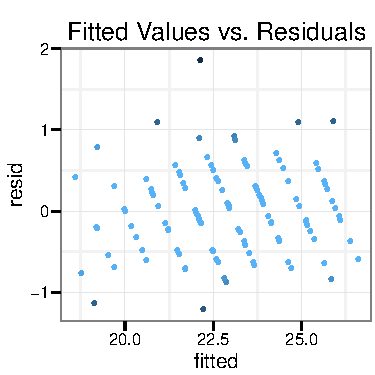
\includegraphics[width=0.45\textwidth]{figs/fig-ex-penicillin-ta}
  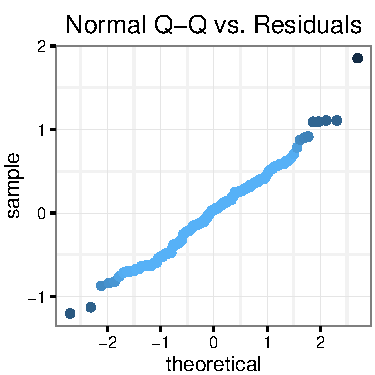
\includegraphics[width=0.45\textwidth]{figs/fig-ex-penicillin-qq-resid}
  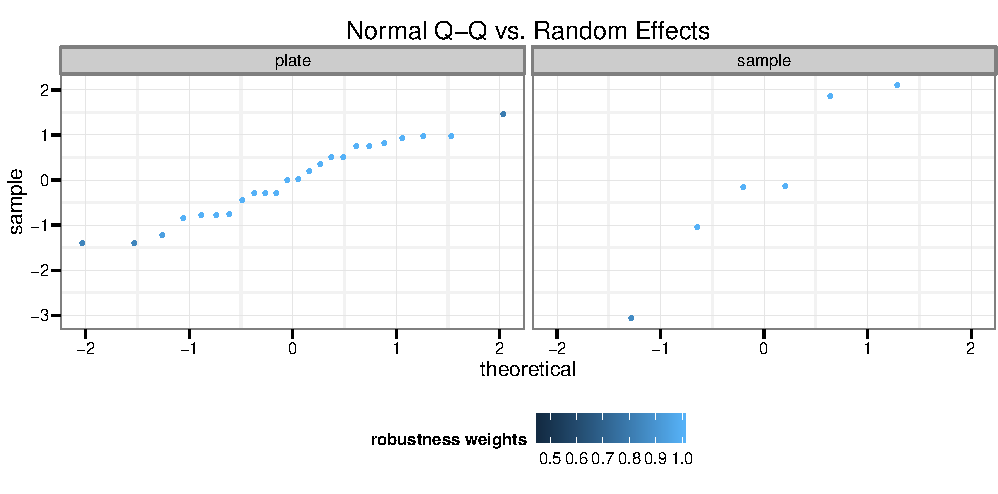
\includegraphics[width=0.9\textwidth]{figs/fig-ex-penicillin-qq-ranef}
  \caption{Residual analysis plots for the ``robust'' object of the
    Penicillin example.}
  \label{fig:penicillinResidualAnalysis}
\end{figure}


\begin{figure}[htb]
  \centering
  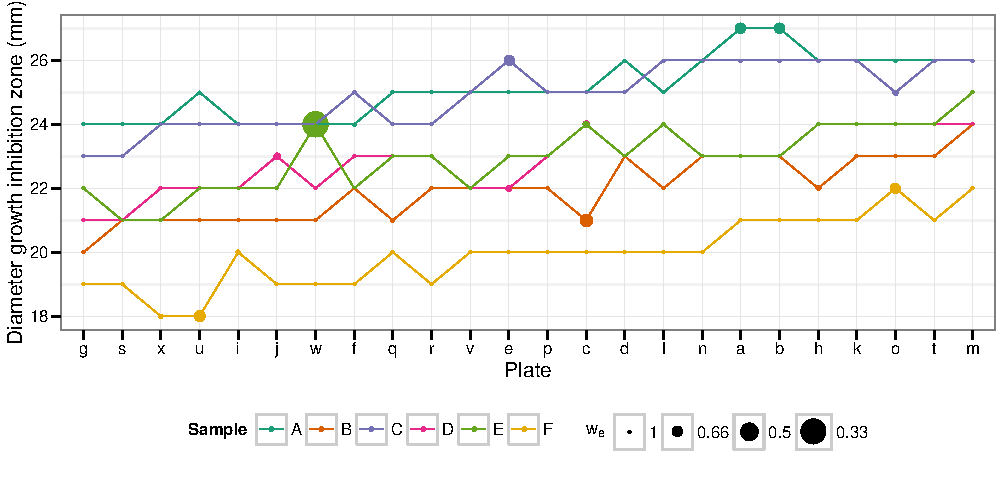
\includegraphics{figs/fig-ex-penicillin-robustness-weights}
  \caption{Diameters of growth inhibition zones of 6 samples applied to
    each of 24 agar plates to assess penicillin concentration in the
    \emph{B. subtilis} method. The lines join the observations of the same
    sample. The plates have been reordered by their means. The sizes of the
    data points show the robustness weights.}
  \label{fig:penicillinRobustnessWeights}
\end{figure}

The results of the three fits are summarized in
Table~\ref{tab:cmpPenicillin}. The differences are minimal. Interestingly,
the estimated variance for ``sample'' is a little smaller for ``robust2''
than for ``robust''. The common residual analysis plots, Tukey-Anscombe
and qq-normal, are shown in Figure~\ref{fig:penicillinResidualAnalysis} for
the ``robust'' object. The points that got a lower robustness weight are
indicated by a darker color. The rest of the observations seem to follow
the central model quite nicely. In Figure~\ref{fig:penicillinRobustnessWeights}
we again show a plot of the data, this time highlighting the observations
that got a low robustness weight.

\section{Sleepstudy Example}
\label{sec:sleepstudy}

This dataset is a subset of data gathered by \citet{belenky03sleepstudy}
for a study of the effects of sleep deprivation time. The $18$ subjects
were chosen from a population of long distance drivers that were allowed to
sleep for only three hours each night. Each subject's reaction time was
measured several times on each day of the trial. The measurements were made
over a course of $10$ days. The data are shown in
Figure~\ref{fig:sleepstudyRaw}.


\begin{figure}[htbp]
  \centering
  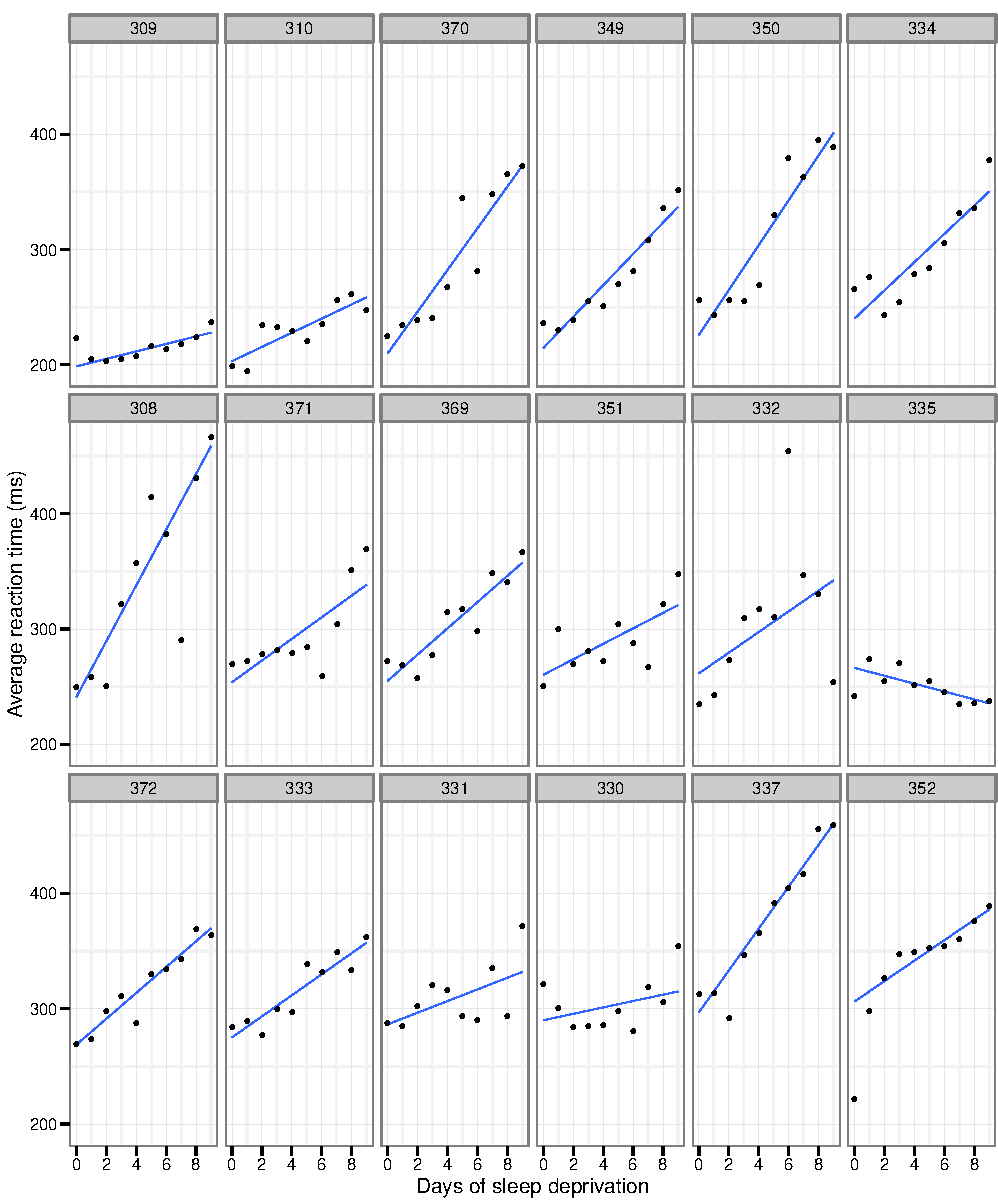
\includegraphics{figs/fig-ex-sleepstudy-raw}
  \caption{The average reaction time of subjects versus days of sleep
    deprivation. Each subject is shown in a separate facet. The lines show
    the robust linear regression fit to the subject's data. The subjects
    have been ordered by increasing intercept. The robust fits were
    computed using the method \emph{lmrob} of the \Rp package
    \emph{robustbase} \citep{robustbase} using \emph{setting=''KS2011''}.}
  \label{fig:sleepstudyRaw}
\end{figure}

The data.frame consists of three columns:

\begin{Schunk}
\begin{Sinput}
> str(sleepstudy)
\end{Sinput}
\begin{Soutput}
'data.frame':	180 obs. of  3 variables:
$ Reaction: num 250 259 251 321 ...
$ Days : num 0 1 2 3 4 5 6 7 ...
$ Subject : Factor w/ 18 levels "309","310","370",..: 7 7 7 7 7 7 7 7 ...
\end{Soutput}
\end{Schunk}

As in \citet{bates2011lme4}, we will fit a random intercept and slope
model. This is an extension of a linear regression model with \T{Reaction}
as response and \T{Days} as predictor. In this model, the coefficients for
each subject are split into a population average (fixed) and a subject
specific (random) part.

The calls to ``lmer'' and ``rlmer'' are quite similar. This time, we omit
the optional ``1'' for the intercept in both the fixed and the random
part. The random effect specification \T{(Days|Subject)} is interpreted as
\T{(1+Days|Subject)}. Specified in this way, the fitted model also
includes a correlation term. To get uncorrelated random effects, one would
have to use two terms, namely \T{(1|Subject) + (0+Days|Subject)}. The \T{0}
tells the method not to include an intercept term. Since the random effects
now have a non-diagonal covariance matrix $\Ubth$, we have to use another
tuning constant for ``rho.sigma.b''. It corresponds roughly to the square
of the one used in the diagonal case.

\begin{Schunk}
\begin{Sinput}
> st(classical <- lmer(Reaction ~ Days + (Days|Subject), sleepstudy))
\end{Sinput}
\end{Schunk}
\begin{Schunk}
\begin{Soutput}
   user  system elapsed 
  0.084   0.001   0.084 
\end{Soutput}
\end{Schunk}
\begin{Schunk}
\begin{Sinput}
> st(robust <-
+    rlmer(Reaction ~ Days + (Days|Subject), sleepstudy,
+          rho.sigma.e = psi2propII(smoothPsi, k = 2.28),
+          rho.sigma.b = chgDefaults(smoothPsi, k = 5.11, s=10)))
\end{Sinput}
\begin{Soutput}
    user   system  elapsed 
1405.825    2.872 2237.468 
\end{Soutput}
\begin{Sinput}
> summary(robust)
\end{Sinput}
\begin{Soutput}
Robust linear mixed model fit by DAStau 
Formula: Reaction ~ Days + (Days | Subject) 
   Data: sleepstudy 

Random effects:
 Groups   Name        Variance Std.Dev. Corr  
 Subject  (Intercept) 784.05   28.001         
          Days         41.68    6.456   -0.037
 Residual             404.16   20.104         
Number of obs: 180, groups: Subject, 18

Fixed effects:
            Estimate Std. Error t value
(Intercept)  252.090      7.295   34.55
Days          10.827      1.646    6.58

Correlation of Fixed Effects:
     (Intr)
Days -0.121

Robustness weights for the residuals: 
 155 weights are ~= 1. The remaining 25 ones are summarized as
   Min. 1st Qu.  Median    Mean 3rd Qu.    Max. 
  0.204   0.597   0.725   0.687   0.872   0.977 

Robustness weights for the random effects: 
 24 weights are ~= 1. The remaining 12 ones are summarized as
   Min. 1st Qu.  Median    Mean 3rd Qu.    Max. 
  0.631   0.692   0.723   0.735   0.742   0.901 

Rho functions used for fitting:
  Residuals:
    eff: smoothed Huber (k = 1.345, s = 10) 
    sig: smoothed Huber, Proposal II (k = 2.28, s = 10) 
  Random Effects, variance component 1 (Subject):
    eff: smoothed Huber (k = 1.345, s = 10) 
    vcp: smoothed Huber (k = 5.11, s = 10) 
\end{Soutput}
\end{Schunk}

The residual analysis plots are shown in
Figure~\ref{fig:sleepstudyResidualAnalysis}. There are some points that are
outside the bulk of the residuals and accordingly get quite a low
robustness weight. The qq-plot of the random effects shows some structure,
but admittedly, the sample size of $18$ is quite low.

\begin{figure}[htbp]
  \centering
  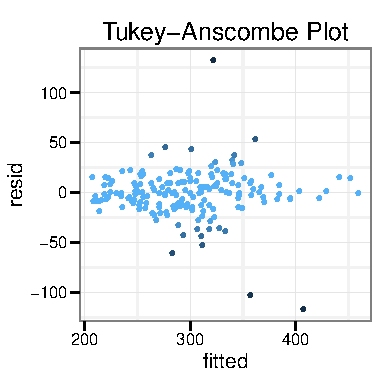
\includegraphics[width=0.45\textwidth]{figs/fig-ex-sleepstudy-ta}
  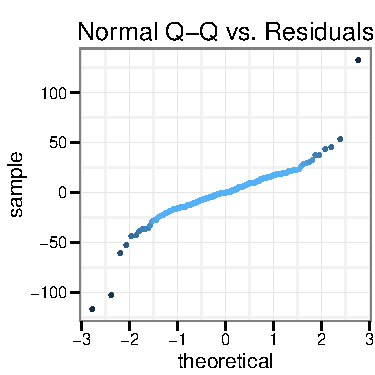
\includegraphics[width=0.45\textwidth]{figs/fig-ex-sleepstudy-qq-resid}
  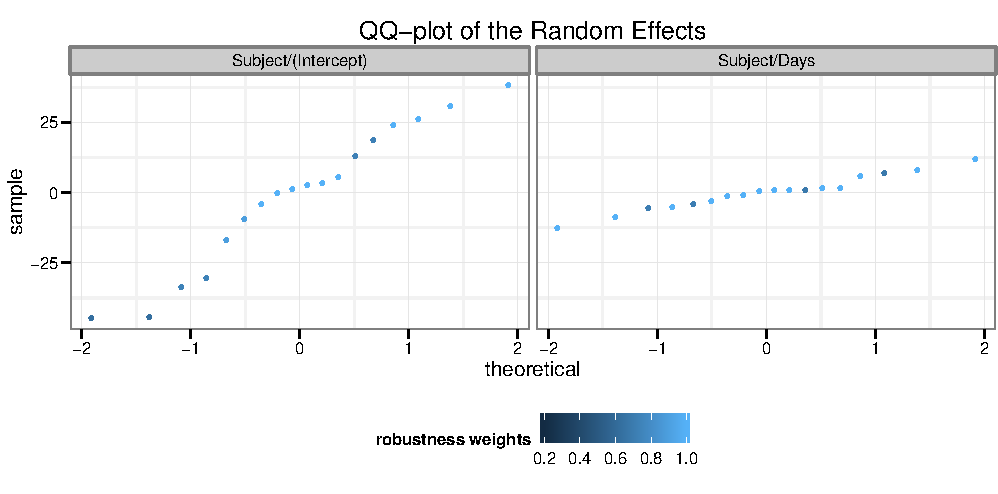
\includegraphics[width=0.9\textwidth]{figs/fig-ex-sleepstudy-qq-ranef}
  \caption{Residual analysis plots for robust fit ``robust'' of the
    Sleepstudy example.}
  \label{fig:sleepstudyResidualAnalysis}
\end{figure}


\begin{figure}[htpb]
  \centering
  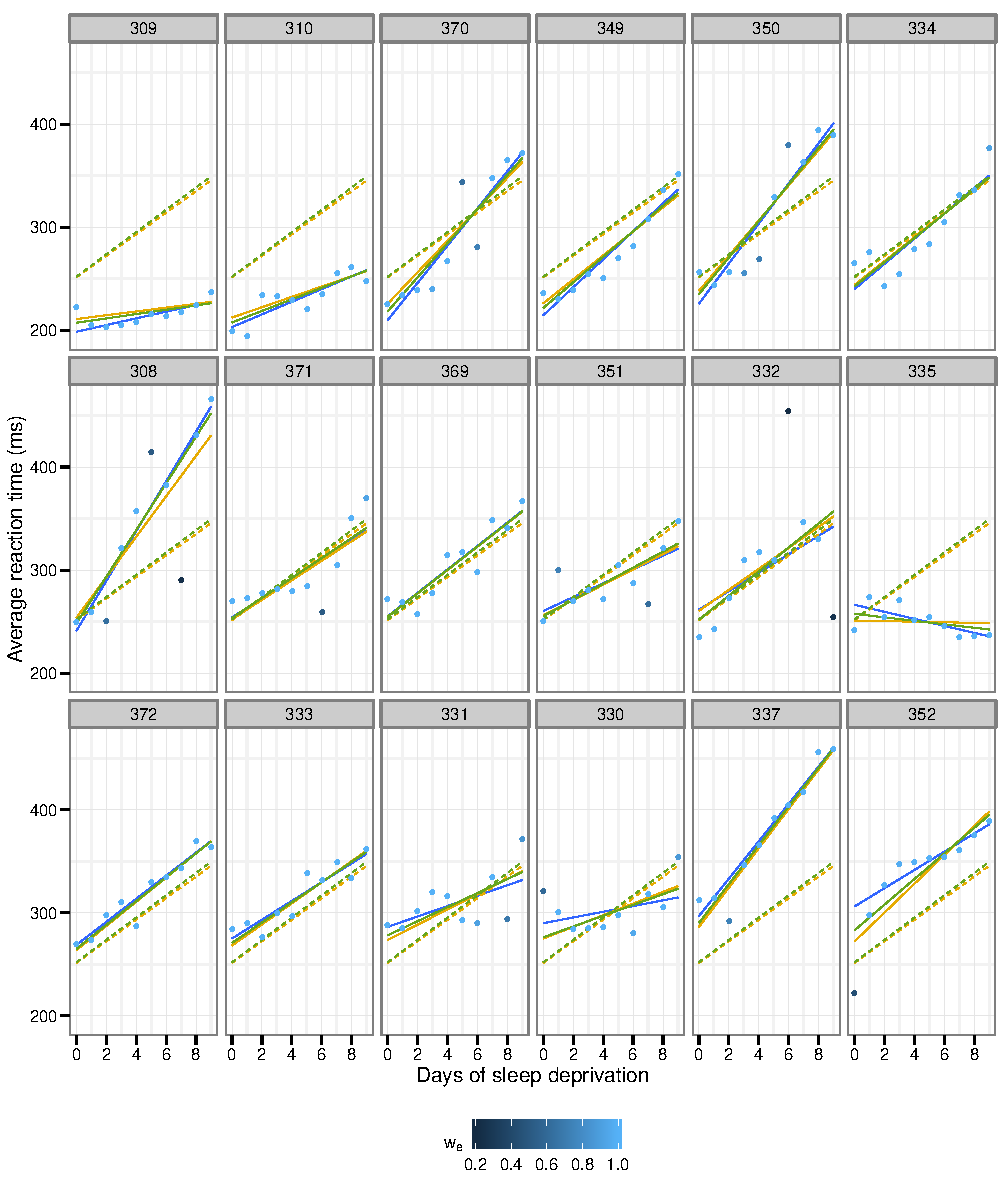
\includegraphics{figs/fig-ex-sleepstudy-ex-comparsion}
  \caption{The average reaction time of subjects versus days of sleep
    deprivation. Each subject is shown in a separate facet. The blue lines
    show the robust linear regression fit to the subject's data. The yellow
    lines show the fitted values of the classical mixed effects model
    including random effects. The green lines show the corresponding robust
    linear mixed effects fit. The dashed lines show the population wide
    fit, robust and classical methods almost coincide. The subjects have
    been ordered by increasing intercept. The robust linear regression fits
    were computed using the method \emph{lmrob} of the \Rp package
    \emph{robustbase} \citep{robustbase} using \emph{setting=''KS2011''}. }
  \label{fig:sleepstudyExComparison}
\end{figure}


\begin{figure}[htb]
  \centering
  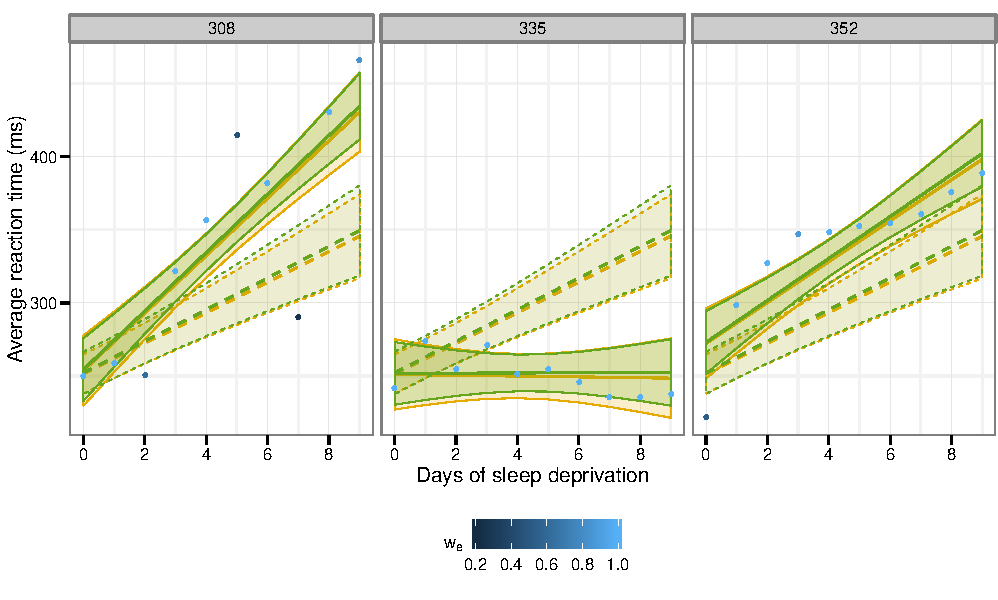
\includegraphics{figs/fig-ex-sleepstudy-ex-comparsion-subsample}
  \caption{The average reaction time of selected subjects versus days of sleep
    deprivation. Additional to the features shown also in
    Figure~\ref{fig:sleepstudyExComparison}, we show the pointwise
    $95\%$ confidence intervals for the fitted values. For better
    visibility, we omit the linear regression fit and show only the three
    subjects with the most pronounced differences between classical and
    robust fits.}
  \label{fig:sleepstudyExComparisonSubsample}
\end{figure}

The fitted values for classical and the robust fits as well as the robust
per-subject fit are shown in Figure~\ref{fig:sleepstudyExComparison}. While
most of the subjects follow the general population fit quite closely,
others, such as subject 335, show even a negative trend. Nevertheless, the
robustness weights for the random effects do not show any clear
outliers. The lowest robustness weight is assigned to subject
$309$ while subject $335$ is given a weight of
$0.69$. The three subjects with the most notable
difference between classical and robust fit are shown again in
Figure~\ref{fig:sleepstudyExComparisonSubsample}. The differences in
Subject $308$ are most pronounced. The predicted slope of the classical fit
is pulled downwards, causing the observations to lie outside or just at the
border of the estimated confidence intervals. The confidence intervals for
the population level estimates of the robust and classical fit are very
similar. Compared to the total number of observations, there are only a
very little observations with a low robustness weight. They are most
probably not able to increase the variance components estimates.

We may check this statement by fitting the same model with redescending
$\psi$-functions. As initial estimate, we use the values of the above
robust fit. With ``rlmer'', one can do this conveniently by using the
``update'' function and specifying redescending $\psi$-functions. The
object that is being updated will be used as initial fit.

%% eff computed: for s=2: c(1.63, 1.09, 1.5) (rho.b)
\begin{Schunk}
\begin{Sinput}
> st(redesc <-
+    update(robust, rho.e = chgDefaults(lqqPsi, cc=c(1.47, 0.98, 1.5)),
+           rho.sigma.e = chgDefaults(lqqPsi, cc=c(2.19, 1.46, 1.5)),
+           rho.b = chgDefaults(lqqPsi, cc=c(1.47, 0.98, 1.5)),
+           rho.sigma.b = chgDefaults(lqqPsi, cc=c(5.95, 3.97, 1.5))))
\end{Sinput}
\begin{Soutput}
    user   system  elapsed 
2991.906    4.851 3002.041 
\end{Soutput}
\begin{Sinput}
> summary(redesc)
\end{Sinput}
\begin{Soutput}
Robust linear mixed model fit by DAStau 
Formula: Reaction ~ Days + (Days | Subject) 
   Data: sleepstudy 

Random effects:
 Groups   Name        Variance Std.Dev. Corr  
 Subject  (Intercept) 809.17   28.446         
          Days         43.66    6.607   -0.069
 Residual             399.39   19.985         
Number of obs: 180, groups: Subject, 18

Fixed effects:
            Estimate Std. Error t value
(Intercept)  251.775      7.435   33.86
Days          10.822      1.690    6.40

Correlation of Fixed Effects:
     (Intr)
Days -0.146

Robustness weights for the residuals: 
 143 weights are ~= 1. The remaining 37 ones are summarized as
   Min. 1st Qu.  Median    Mean 3rd Qu.    Max. 
 0.0118  0.6730  0.8890  0.7820  0.9800  0.9990 

Robustness weights for the random effects: 
 14 weights are ~= 1. The remaining 22 ones are summarized as
   Min. 1st Qu.  Median    Mean 3rd Qu.    Max. 
  0.690   0.778   0.929   0.879   0.977   0.995 

Rho functions used for fitting:
  Residuals:
    eff: lqq (cc1 = 1.47, cc2 = 0.98, cc3 = 1.5) 
    sig: lqq (cc1 = 2.19, cc2 = 1.46, cc3 = 1.5) 
  Random Effects, variance component 1 (Subject):
    eff: lqq (cc1 = 1.47, cc2 = 0.98, cc3 = 1.5) 
    vcp: lqq (cc1 = 5.95, cc2 = 3.97, cc3 = 1.5) 
\end{Soutput}
\end{Schunk}
% latex table generated in R 3.0.1 by xtable 1.7-1 package
% Mon Jun 17 09:45:07 2013
\begin{table}[ht]
\centering
{\small
\begin{tabular}{rlll}
  \hline
  & classical & robust & redesc \\ 
  \hline
Coefficients (Std. Error) &  &  &  \\ 
  (Intercept) & 251.4 (6.82) & 252.1 (7.30) & 251.8 (7.44) \\ 
  Days &  10.5 (1.55) &  10.8 (1.65) &  10.8 (1.69) \\ 
   \hline
Variance components &  &  &  \\ 
  (Intercept) $|$ Subject & 24.74 & 28.00 & 28.45 \\ 
  Days $|$ Subject &  5.92 &  6.46 &  6.61 \\ 
   \hline
Correlations &  &  &  \\ 
  (Intercept) $\times$ Days $|$ Subject &  0.0656 & -0.0369 & -0.0695 \\ 
   \hline
$\sigma$ & 25.6 & 20.1 & 20 \\ 
   \hline
REML & 1744 &  &  \\ 
   \hline
\end{tabular}
}
\caption{Comparison table of the fitted models for the Sleepstudy example.} 
\label{tab:cmpSleepstudy}
\end{table}
A comparison table of the three fits is shown in
Table~\ref{tab:cmpSleepstudy}. The two robust fits are quire similar. The
variance attributed to the between subjects effects is a little lower for
the fit using redescending $\psi$-functions, while the two estimates of the
residual standard errors are almost identical. We therefore conclude that
the few observations with a small robustness weight were not able to unduly
increase the estimates residual standard error.  While the estimated
residual standard errors for both robust fits are smaller than for the
classical fit, the estimated standard errors of the fixed effects estimates
are a little increased (the estimated standard error for the classical fit
is $6.82$ for the intercept and
$1.55$ for ``Days'').

The robust fits return a negative estimate of the correlation between the
random intercept and slopes. When choosing smaller tuning parameters for
the functions ``rho.b'' and ``rho.sigma.b'', the correlation is estimated
even lower. A scatterplot of the estimated random effects is shown in
Figure~\ref{fig:ranefSleepstudy}. With help from the coloring of the
points, one can see a hint of a negative correlation between the two random
effects (suppressing the points below and above the falling diagonal). This
is picked up by the estimator. For smaller tuning parameters, the weight
function decreases more quickly and the off-diagonal points get a lower
weight, finally this leads to a negative estimate of the correlation.


\begin{figure}[htb!]
  \centering
  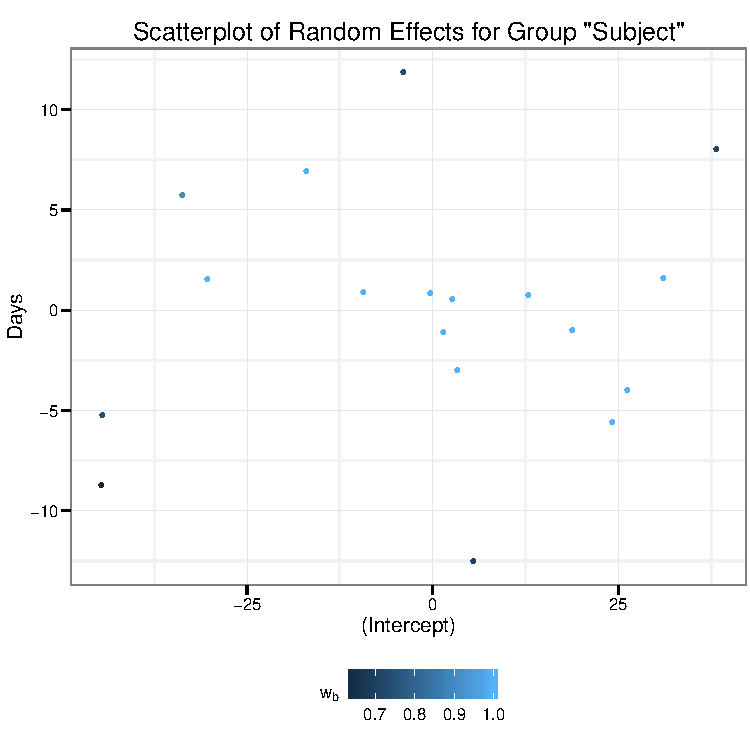
\includegraphics[width=0.75\textwidth]{figs/fig-ex-sleepstudy-ranef-scatterplot}
  \caption{Scatterplot of the estimated random effects for the ``redesc''
    fit for the Sleepstudy example using redescending lqq
    $\psi$-functions.}
  \label{fig:ranefSleepstudy}
\end{figure}

% We show the residual analysis plots for the redescending fit in
% Figure~\ref{fig:sleepstudyResidualAnalysisRedescending}. The outlying point
% now have an even lower robustness weight, some of them almost zero. The
% QQ-plots for the random effects do not show the structure anymore.

% <<sleepstudy-redesc-ta,fig=TRUE,width=2.5,height=2.5>>=
% robust.bak <- robust
% robust <- redesc
% <<penicillin-ta>>
% <<sleepstudy-redesc-qq-resid,fig=TRUE,width=2.5,height=2.5>>=
% <<penicillin-qq-resid>>
% <<sleepstudy-redesc-qq-ranef,fig=TRUE,height=3.3>>=
% <<penicillin-qq-ranef>>
% robust <- robust.bak
% @

% \begin{figure}[htbp]
%   \centering
%   \includegraphics[width=0.45\textwidth]{figs/fig-ex-sleepstudy-redesc-ta}
%   \includegraphics[width=0.45\textwidth]{figs/fig-ex-sleepstudy-redesc-qq-resid}
%   \includegraphics[width=0.9\textwidth]{figs/fig-ex-sleepstudy-redesc-qq-ranef}
%   \caption{Residual analysis plots for robust fit ``redesc'' of the
%     Sleepstudy example using the lqq $\psi$-function.}
%   \label{fig:sleepstudyResidualAnalysisRedescending}
% \end{figure}

\clearpage
\section{$\psi$-functions and Tables of Tuning Constants}
\label{sec:tc}
The \emph{smoothed Huber $\psi$-function} is defined as
\begin{equation}
  \psi(x, k, s) = \left\{
    \begin{array}{ll}
      x & \abs{x} \leq c \\
      \sign(x)\left(k - \frac{1}{(\abs{x}-d)^{s}}\right) &
      \mbox{otherwise}
    \end{array}
  \right.\;,
\end{equation}
where $c = k - s^{\frac{-s}{s+1}}$ and $d = c - s^{\frac{1}{s+1}}$. We have
always used $s = 10$ for our simulations. With this value, the asymptotic
properties of the regular Huber function and the smoothed Huber function
are almost identical. We can therefore safely use the same tuning parameter
$k$ for both $\psi$-functions. A comparison of the two $\psi$-functions is
shown in Figure~\ref{fig:smoothedHuber}. Useful tables of tuning constants
for this and the lqq $\psi$-function are given in Tables
\ref{tab:tuningParameters} to \ref{tab:effLqq}.


\vspace{5ex}

\begin{figure}[htbp!]
  \centering
  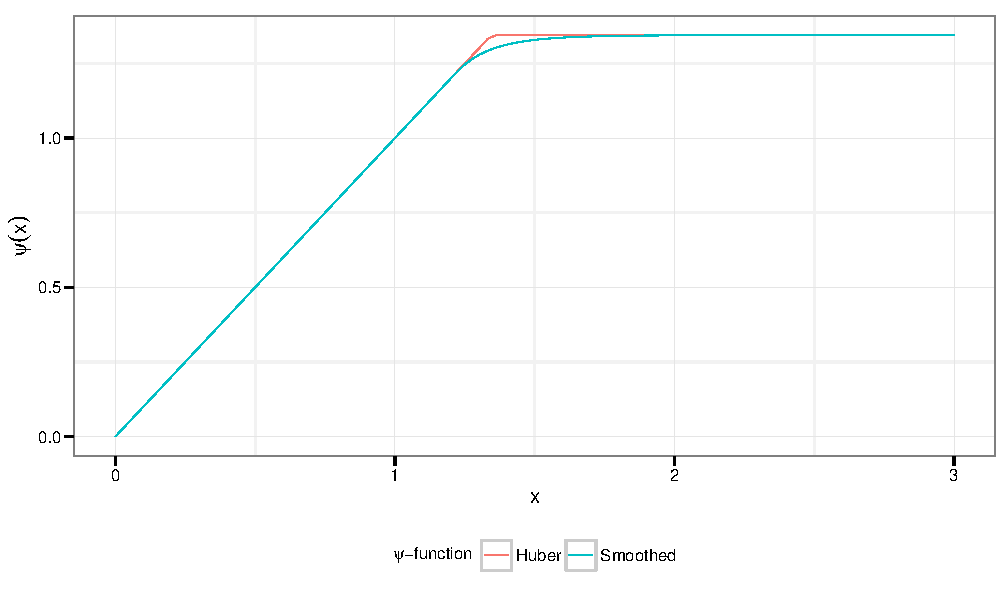
\includegraphics{figs/fig-ex-smoothedHuber}
  \caption{Comparison of the Huber and the smoothed Huber $\psi$-function
    for $k = 1.345$ and $s = 10$.}
  \label{fig:smoothedHuber}
\end{figure}

%% functions required to compute efficiencies

\clearpage
\begin{table}[htbp]
  \centering
  % latex table generated in R 2.15.2 by xtable 1.7-0 package
% Wed Dec 12 11:31:41 2012
{\small
\begin{tabular}{lccc}
  \hline
efficiency & $k$ for $\hat\mu$ & $k$ for $\hat\sigma_\text{\eqref{eq:sigmaDAS}}$ & $k$ for $\hat\sigma_\text{\eqref{eq:sigmaDAS}}$, Prop. II \\ 
  \hline
  0.80 & 0.53  & 0.50 & 1.49 \\ 
  0.85 & 0.73  & 0.71 & 1.69 \\ 
  0.90 & 0.98  & 1.08 & 1.94 \\ 
  0.95 & 1.345 & 1.66 & 2.28 \\ 
   \hline
\end{tabular}
}

  \caption{Tuning parameters $k$ for scale estimates such that they reach the
    same asymptotic efficiency as the location estimate. For the Huber
    $\psi$-function.}
  \label{tab:tuningParameters}
\end{table}

% latex table generated in R 2.15.2 by xtable 1.7-0 package
% Mon Nov 26 15:25:38 2012
\begin{table}[htbp!]
\begin{center}
{\small
\begin{tabular}{rllllll}
   \hline
  & \multicolumn{5}{c}{dimension $s$} \\
  \cline{2-7}
  & 2 & 3 & 4 & 5 & 6 & 7 \\
   \hline
$b_\eta$ & 5.66 & 6.41 & 7.14 & 7.87 & 8.58 & 9.28 \\
  $b_\tau$ & 5.15 & 5.55 & 5.91 & 6.25 & 6.55 & 6.84 \\
  $b_\mu$ & 1.5 & 1.63 & 1.73 & 1.81 & 1.87 & 1.9 \\
   \hline
\end{tabular}
}
\caption{Tuning parameters for the optimal $B$-estimator to yield $95\%$
  efficiency, non-diagonal case. For the Huber $\psi$-function.}
\label{tab:effBOptimal}
\end{center}
\end{table}

% latex table generated in R 2.15.2 by xtable 1.7-0 package
% Wed Dec 12 10:11:41 2012
\begin{table}[htbp!]
\begin{center}
{\small
\begin{tabular}{lll}
  \hline
efficiency & $cc$ for $\hat\mu$ & $cc$ for $\hat\sigma_\text{\eqref{eq:sigmaDAS}}$ \\ 
  \hline
0.80 & ($0.946$,$0.631$) & ($1.414$,$0.942$) \\ 
  0.85 & ($1.058$,$0.705$) & ($1.57$,$1.05$) \\ 
  0.90 & ($1.214$,$0.809$) & ($1.79$,$1.19$) \\ 
  0.95 & ($1.474$,$0.982$) & ($2.19$,$1.46$) \\ 
   \hline
\end{tabular}
}
\caption{Tuning parameters for lqq $\psi$-function for the location and scale estimates such that they reach the given asymptotic efficiency. The third parameter is always taken to be $1.5$.}
\label{tab:eqqLqqLocationScale}
\end{center}
\end{table}

% latex table generated in R 2.15.2 by xtable 1.7-0 package
% Mon Nov 26 15:26:18 2012
\begin{table}[htbp!]
\begin{center}
{\small
\begin{tabular}{rlllll}
  \hline
  & \multicolumn{5}{c}{dimension $s$} \\
  \cline{2-6}
   & 2 & 3 & 4 & 5 & 6 \\
   \hline
$cc_\eta$ & ($6.44$,$4.29$) & ($7.23$,$4.82$) & ($8.01$,$5.34$) & ($8.77$,$5.85$) & ($9.52$,$6.35$) \\
  $cc_\tau$ & ($5.95$,$3.97$) & ($6.41$,$4.27$) & ($6.82$,$4.55$) & ($7.2$,$4.8$) & ($7.55$,$5.03$) \\
  $cc_\mu$ & ($1.63$,$1.09$) & ($1.77$,$1.18$) & ($1.88$,$1.26$) & ($1.99$,$1.32$) & ($2.08$,$1.39$) \\
   \hline
\end{tabular}
}
\caption{Tuning parameters for the lqq weight function to yield $95\%$
  efficiency, non-diagonal case. The third parameter is always taken to be $1.5$.}
\label{tab:effLqq}
\end{center}
\end{table}


\clearpage
\addcontentsline{toc}{chapter}{Bibliography}
\bibliographystyle{apalike}
\bibliography{rlmer}


\end{document}
